\chapter{Compiler Spezifikation}
\label{chap:CompilerEntwurf}
Zur Entwicklung eines möglichst effektiven Compilers ist es notwendig, die genauen Anforderungen zu ermitteln,  um dann passende Softwaretechnische Lösungen zu erarbeiten. \footcite[Vgl.][S.6]{Balzert2011} Im speziellen Falle besteht die Anforderung darin, vom Quellframework Xamarin.Forms in das Zielframework Flutter zu übersetzen,  welche beide für die Entwicklung von plattformunabhängigen Smartphone-Apps verwendet werden können.  Für eine genaue Spezifikation des zu realisieren Source-To-Source Compilers ist es notwendig, einen Überblick über das Compiler-Umfeld zu erhalten.  Dieses wird in Abbildung \ref{fig:CompilerArchitecture} visualisiert. 

\begin{figure}[!ht]
 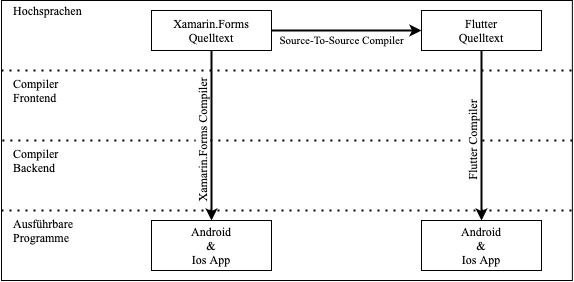
\includegraphics[width=\textwidth,keepaspectratio]{Images/CompilerArchitecture/CompilerStructure.png}
 \caption{Umfeld des Source-To-Source Compilerns}
 \label{fig:CompilerArchitecture}
\end{figure}

Wie auf der Abbildung erkennbar ist,  durchlaufen sowohl Xamarin.Forms als auch Flutter bei der Übersetzung zu mobilen Anwendungen die in Kapitel \ref{fig:S2SCompilerAufbau} erläuterten Phasen,  kurz dargestellt als Compiler Front- und Backend.  Der Source-To-Source Compiler ist in der Abbildung horizontal dargestellt,  was veranschaulichen soll,  dass sich sowohl die Quelle,  als auch das Ziel der Übersetzung auf einer Abstraktionsebene befinden.  Auch bei dieser Übersetzung sind die Compilerphasen aus dem vorherigen Kapitel anzuwenden.  So lässt sich die Abbildung \ref{fig:CompilerArchitecture},  wie in \ref{fig:S2SCompilerAufbau} dargestellt, um ein Front- und Backend erweitern.

\begin{figure}[!ht]
 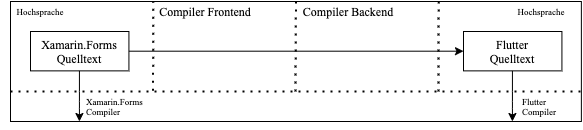
\includegraphics[width=\textwidth,keepaspectratio]{Images/CompilerArchitecture/S2SArchitecture.png}
 \caption{Source-To-Source Compiler Aufbau}
 \label{fig:S2SCompilerAufbau}
\end{figure}

Laut Definition von Compilern, erzeugen diese ein gleichwertiges Programm in einer Zielsprache.  Sowohl Xamarin.Forms als auch Flutter stellen mit Hilfe ihrer Compiler gleichwertige Programme in Form von mobilen Apps dar.  Da der Source-to-Source Compiler ebenfalls eine gleichwertige Darstellung erzeugt, ist anzunehmen, dass die übersetzte Ursprungs-App gleichwertig zu der übersetzten Flutter App ist. 

\section{Funktionseingrenzung}
Zur Beantwortung der Forschungsfrage ist es ausreichend, dass der Prototyp einen begrenzten Funktionsumfang hat.  Für eine zielführende Eingrenzung eignen sich die folgenden fünf Aspekte:

\begin{itemize}
\setlength\itemsep{-0.6em}
 \item Framework Version: Der in dieser Arbeit zu realisierende Prototyp soll ausschließlich das offiziell von Microsoft veröffentliche Xamarin.Forms in der Version 5.0.0.2012 zu Flutter übersetzten.  
 \item Erweiterungen von Dritten: Viele Firmen und einzelne Entwickler haben Erweiterungen für Xamarin.Forms programmiert.  Aufgrund der großen Anzahl und stetigen Veränderung dieser Erweiterungen, werden sie in dieser Arbeit nicht weiter betrachtet.  
 \item Plattformspezifischer Quelltext: Xamarin.Forms erlaubt die Verwendung von plattformspezifischem Quelltext,  der in dieser Arbeit keine Beachtung finden wird, da eine gleichwertige Darstellung in Flutter nicht garantiert werden kann. 
  \item \ac{ui}: Für die Entwicklung von Benutzeroberflächen kann die Programmiersprache \Csharp verwendet werden,  jedoch hat die Alternative \ac{xaml} für Entwickler Vorteile, \footcite[Vgl.][Abgerufen am \today]{MicrosoftXAML2017} weswegen die Konstruktion von Benutzeroberflächen mit \Csharp in dieser Arbeit nicht berücksichtigt wird.  
  \item App-Styles: Für die visuelle Darstellung wird in dieser Arbeit ausschließlich das Design-System Material von Google unterstützt.  Da die Übersetzung von Darstellungsoptionen sehr aufwendig ist,  und für den in dieser Arbeit zu entwickelnden Prototypen nicht notwendig ist.  
\end{itemize}

Diese Eingrenzungen führen in Summe zu einer Vielzahl von nicht in Gänze übersetzbaren Xamarin.Forms Anwendungen.  Durch Erweiterungen des Compilers könnte diese Limitierung in Zukunft aufgehoben werden.  Im Rahmen dieser Arbeit wird eine mobile Xamarin.Forms Anwendung entworfen, die vollständig übersetzt werden kann, da sie keine der oben definierten Ausschlüsse verwendet. 


\section{Übersetzung von verschiedenen Dateien}
Durch seinen modularen Aufbau, kann der im letzten Kapitel eingeführte Roslyn Compiler die Phasen bis zur semantischen Analyse im zu entwickelnden Prototypen übernehmen.  Anschließend kann mithilfe des dabei typisierten Syntaxbaumes die Übersetzung in die Zielsprache durchgeführt werden.   Die Übersetzung mit Roslyn hat Grenzen,  die aus der Zusammensetzung von Xamarin.Forms Projekten resultiert.  Wie in Abbildung \ref{fig:CompilerStruktur} zu erkennen ist,  setzten sich Xamarin.Forms Projektmappen aus verschiedenen Dateien zusammen, von denen ausschließlich die Klassen beinhaltenden Dateien mit der Endung \glq cs\grq{}  analysiert werden können. 

\begin{figure}[!ht]
 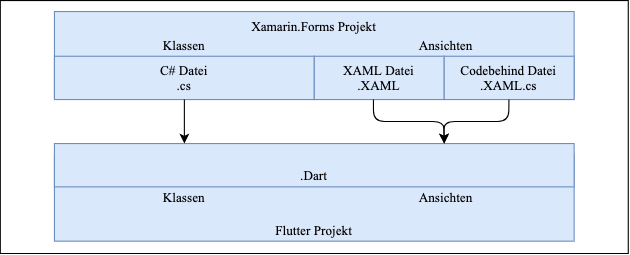
\includegraphics[width=14.5cm]{Images/Compiler/CompilerArchitecture.png}
 \caption{Compiler-Struktur}
 \label{fig:CompilerStruktur}
\end{figure}

Neben den Klassen zeigt die Abbildung \ref{fig:CompilerStruktur},  dass auch Ansichten ein Teil von Xamarin.Forms Projekten sind.  Diese bestehen aus \glq XAML\grq{}  sowie \glq XAML.cs\grq{}  Dateien.  Alle Ausgangsdateien müssen zu Dart-Dateien kompiliert werden,  um ein Flutter Projekt als Ziel zu ergeben.  Die Zusammenführung von \glq XAML\grq{}  und \glq XAML.cs\grq{} Dateien ist dabei notwendig,  weil Flutter ohne sogenannte Codebehind Dateien auskommt. 

\section{Informationsfluss}


\section{Grafische Darstellung}
Damit Unternehmen und Entwickler ihre bestehenden Xamarin.Forms Anwendungen übersetzen können, muss eine Möglichkeit für die Interaktion mit dem Source-To-Source Compiler existieren.  Dieser Compiler ist zur einmaligen und nicht regelmäßigen Verwendung ausgelegt und braucht somit nicht in einer Entwicklungsumgebung integrieren werden.  Der Roslyn Compiler ist ausschließlich für das Betriebssystem Windows verfügbar,  die zu entwickelnde Oberfläche muss dementsprechend auf Windows Computern lauffähig sein.  Abbildung \ref{fig:UiMockup} zeigt einen Entwurf (engl. Mockup) der geplanten \ac{gui}.

\begin{figure}[!ht]
 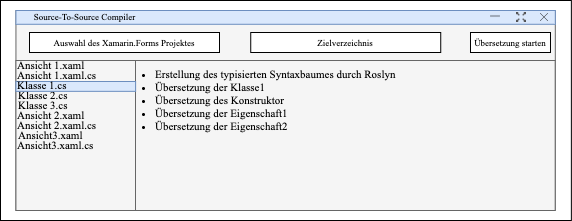
\includegraphics[width=\textwidth,keepaspectratio]{Images/CompilerArchitecture/Mockup.png}
 \caption{Mockup der grafischen Oberfläche}
 \label{fig:UiMockup}
\end{figure}

Im oberen Teil der GUI befindet sich eine Auswahl für das Quellprojekt und das Zielverzeichnis des Compilers.  Der untere Teil der Ansicht zeigt die Ausgabe des Übersetzers,  für die im linken Bereich alle bearbeiteten Dateien angezeigt werden.  Bei der Auswahl einer Datei werden in dem Bereich daneben alle vorgenommen Übersetzungsschritte aufgeführt.

\section{Quelltext Optimierung}
Die Optimierung des Quelltextes ist, wie in Kapitel \ref{chap:Compiler} beschrieben,  eine Phase der Kompilierung.  Im Gegensatz zu den dort beschriebenen Aspekten (Geschwindigkeit und Ressourcenschonung) sind für den Source-To-Source Compiler andere Faktoren wie der Austausch von Klassen und Methoden relevant,  da diese Ressourcenoptimierung später bei der Übersetzung durch den Flutter Compiler stattfinden.   
Der Bedarf zum Austausch von Klassen und Methoden resultiert aus unterschiedlichen Arbeitsweisen der Frameworks,  sodass eine einfache 1:1 Übersetzung nicht möglich ist.  Um dies zu visualisieren, wird folgend ein Quelltextbeispiel aus beiden Frameworks gezeigt,  die die selbe Funktionalität abbilden.

\lstinputlisting[label={lst:XFSelectImage},caption={Bilderauswahl in Xamarin.Forms}, language=csh]{SourceCode/Galery.cs}

\lstinputlisting[label={lst:FlutterSelectImage},caption={Bilderauswahl in Dart}, language=Dart]{SourceCode/Galery.Dart}

Beide Crossplatform Frameworks verwenden in diesem Beispiel unterschiedliche Klassen für die Auswahl eines Bildes aus der Smartphonegalerie.  Daher ist es notwendig,  beide Frameworks zu analysieren und die genauen Unterschiede zwischen den Arbeitsweisen zu verstehen.  Zu diesem Zweck werden im nachfolgenden Kapitel sowohl die Frameworks als auch deren Programmiersprachen analysiert.  Hieraus resultiert das Verständnis, inwiefern sich Benutzeroberflächen und Sprachen unterscheiden und wie diese übersetzt werden können.

Source-To-Source Compiler bilden eine Brücke zwischen zwei Hochsprachen.  Der für die Beantwortung der Forschungsfrage geplante Compiler soll darüber hinaus auch die Arbeitsweisen des Quellprogramms in das Zielprogramm übersetzen.  Das heißt, es soll versucht werden,  ein frameworkbasierte App in die Form eines Zielframeworks zu überführen. 




